% Provenance (never printed): cycle 2 "Questionner l'espace et le temps"
% (the globe, the continents and the oceans, reading a world map); see
% sources/book1/PROVENANCE.md. Book 1, grade 3, chapter 2.
\chapter{De globe: continenten en oceanen}\label{ch:g3:continents-and-oceans}

In het klaslokaal van Lena staat een \omterm{def:g3:continents-and-oceans:globe}{globe} op een voet. Lena doet haar
ogen dicht, laat de \omterm{def:g3:continents-and-oceans:globe}{globe} met één vinger draaien en stopt hem met haar
vingertop. Ze doet haar ogen open: haar vinger staat op blauw, midden in
een \omterm{def:g2:water-on-earth:ocean}{oceaan}. Ze probeert het nog eens: weer blauw. De derde keer komt ze op
geelgroen terecht, ergens midden in Afrika.

Lena speelt door en telt. Haar vinger stopt veel vaker op de \omterm{def:g2:water-on-earth:ocean}{zee} dan op het
land. Waarom? En wat zijn al die vormen van land en water die onder haar
vinger door draaien?

\begin{omfigure}
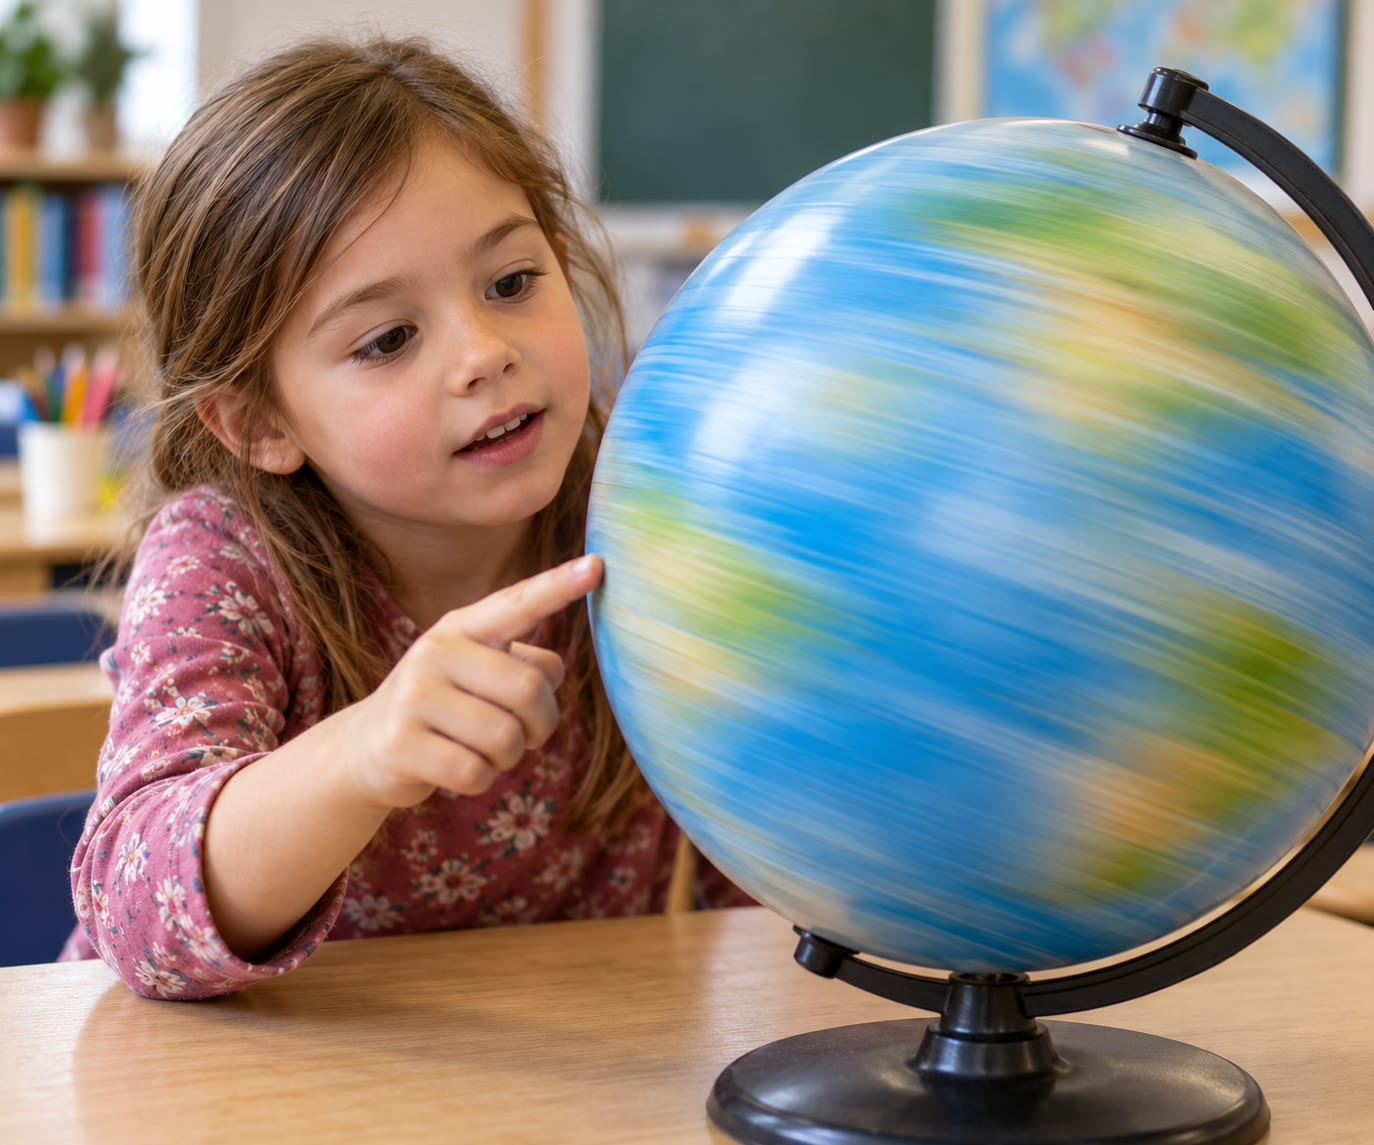
\includegraphics[width=0.6\linewidth]{images/book1/ai/g3-spinning-globe.jpg}

{\small Een \omterm{def:g3:continents-and-oceans:globe}{globe} die op zijn voet draait: land en \omterm{def:g2:water-on-earth:ocean}{zee} schuiven onder de
vinger door.}
\end{omfigure}

\begin{recall}
Het grootste deel van de Aarde is bedekt met \omterm{def:g2:water-on-earth:salt-fresh}{zout water}: ongeveer
71 vierkantjes van de 100 in het rooster van \cref{ch:g2:water-on-earth}.
Een \omterm{def:g2:water-on-earth:ocean}{oceaan} is een heel grote watervlakte met \omterm{def:g2:water-on-earth:salt-fresh}{zout water} tussen de
landmassa's; een \omterm{def:g2:water-on-earth:ocean}{zee} is een kleinere, aan de rand van een \omterm{def:g2:water-on-earth:ocean}{oceaan}. Een \omterm{def:g2:drawing-to-map:map}{kaart}
is een tekening van een plek van bovenaf gezien, kleiner gemaakt
(\cref{ch:g2:drawing-to-map}). De natuurkundeboeken vertellen hoe de Aarde
eens per dag om zichzelf draait, en dat geeft ons dag en nacht.
\end{recall}

\section{De globe, een klein model van de ronde Aarde}

De Aarde is rond, zoals een heel grote bal. Vanaf de grond kunnen we die
vorm niet zien, omdat ze veel te groot is: waar we ook staan, de grond lijkt
vlak. Maar astronauten die ver van de Aarde weg reisden, zagen haar in haar
geheel, een ronde blauwe bal in de zwarte hemel (de foto aan het begin van
\cref{ch:g2:water-on-earth}).

Om de hele Aarde in een klaslokaal te zien, maken we haar klein.

\begin{definition}[Globe]\label{def:g3:continents-and-oceans:globe}
Een \emph{globe}\index{globe} is een model van de Aarde: een bol waarop
het land en de \omterm{def:g2:water-on-earth:ocean}{oceanen} getekend zijn met dezelfde vormen als op de echte
Aarde, alleen veel en veel kleiner.
\end{definition}

Een \omterm{def:g3:continents-and-oceans:globe}{globe} is de beste afbeelding van de Aarde, omdat hij de juiste vorm
heeft: rond. Maar net als van de echte Aarde kunnen we er telkens maar één
helft van zien. Om de andere helft te zien, draaien we hem om.

\begin{omfigure}
\begin{tikzpicture}
\begin{axis}[name=atl, hide axis, axis equal image, scale only axis,
    width=6.2cm, xmin=-1.05, xmax=1.05, ymin=-1.05, ymax=1.05, clip=false]
  \fill[omSea] (axis cs:0,0) circle[radius=1];
  \addplot[fill=omHypsLandA!85!black, draw=black!45, line width=0.2pt]
    table {figdata/out/grade-3-globe-atlantic-land.dat};
  \addplot[black!60, dashed, line width=0.5pt]
    table {figdata/out/grade-3-globe-atlantic-equator.dat};
  \addplot[only marks, mark=*, mark size=1.4pt, black]
    table[x=x, y=y] {figdata/out/grade-3-globe-atlantic-poles.dat};
  \addplot[only marks, mark=none, nodes near coords, point meta=explicit symbolic,
    nodes near coords style={font=\scriptsize, anchor=center, fill=white, fill opacity=0.7, text opacity=1, inner sep=1pt, rounded corners=1pt}]
    table[x=x, y=y, meta=name, row sep=\\] {name x y\\ Noord-Amerika -0.683 0.636\\ Zuid-Amerika -0.561 -0.408\\ Europa 0.396 0.639\\ Afrika 0.704 -0.098\\ Atlantische~Oceaan -0.209 0.128\\ };
  \draw[black!70, line width=0.8pt] (axis cs:0,0) circle[radius=1];
  \node[font=\scriptsize, anchor=south] at (axis cs:0,0.97) {Noordpool};
\end{axis}
\begin{axis}[at={(atl.east)}, anchor=west, xshift=0.6cm, hide axis,
    axis equal image, scale only axis,
    width=6.2cm, xmin=-1.05, xmax=1.05, ymin=-1.05, ymax=1.05, clip=false]
  \fill[omSea] (axis cs:0,0) circle[radius=1];
  \addplot[fill=omHypsLandA!85!black, draw=black!45, line width=0.2pt]
    table {figdata/out/grade-3-globe-pacific-land.dat};
  \addplot[black!60, dashed, line width=0.5pt]
    table {figdata/out/grade-3-globe-pacific-equator.dat};
  \addplot[only marks, mark=none, nodes near coords, point meta=explicit symbolic,
    nodes near coords style={font=\scriptsize, anchor=center, fill=white, fill opacity=0.7, text opacity=1, inner sep=1pt, rounded corners=1pt}]
    table[x=x, y=y, meta=name, row sep=\\] {name x y\\ Australië -0.754 -0.391\\ Stille~Oceaan 0.258 0.087\\ };
  \draw[black!70, line width=0.8pt] (axis cs:0,0) circle[radius=1];
\end{axis}
\end{tikzpicture}

{\small De \omterm{def:g3:continents-and-oceans:globe}{globe} van twee kanten gezien. Links: de kant van de Atlantische
\omterm{def:g2:water-on-earth:ocean}{Oceaan}, met Amerika, Europa en Afrika. Rechts: de andere kant, de Stille
\omterm{def:g2:water-on-earth:ocean}{Oceaan}, met Australië aan de rand. De gestippelde lijn is de \omterm{def:g3:continents-and-oceans:equator}{evenaar}.
Kustlijnen: Natural Earth (publiek domein).}
\label{fig:g3:continents-and-oceans:globes}
% ledger: data:ne-land
\end{omfigure}

\begin{remark}[Twee heel verschillende helften]\label{rem:g3:continents-and-oceans:halves}
Kijk naar de twee afbeeldingen. Links bedekt het land ongeveer 4 delen van
de 10 van het plaatje. Rechts maar ongeveer 1 deel van de 10: de kant van
de Stille \omterm{def:g2:water-on-earth:ocean}{Oceaan} is bijna helemaal water. Als Lena's vinger aan die kant
van de \omterm{def:g3:continents-and-oceans:globe}{globe} stopt, komt hij bijna altijd op de \omterm{def:g2:water-on-earth:ocean}{zee} terecht.
\end{remark}

\section{De evenaar, de polen en de twee halfronden}

Een \omterm{def:g3:continents-and-oceans:globe}{globe} draait om een staaf die er dwars doorheen gaat, van boven naar
onder. De echte Aarde heeft geen staaf, maar ook zij draait om een lijn
door haar midden. De twee plekken waar die lijn uit de Aarde komt, hebben
een naam.

\begin{definition}[Pool]\label{def:g3:continents-and-oceans:poles}
De \emph{Noordpool}\index{Noordpool} en de \emph{Zuidpool}\index{Zuidpool}
zijn de twee punten helemaal boven en helemaal onder op de Aarde, waar de
lijn waar de Aarde om draait naar buiten komt. Elk van beide is een
\emph{pool}\index{pool}. Op een \omterm{def:g3:continents-and-oceans:globe}{globe} ligt de Noordpool bovenaan.
\end{definition}

\begin{definition}[Evenaar en halfrond]\label{def:g3:continents-and-oceans:equator}
De \emph{evenaar}\index{evenaar} is een denkbeeldige lijn die helemaal om
de Aarde heen loopt, precies halverwege de \omterm{def:g3:continents-and-oceans:poles}{Noordpool} en de \omterm{def:g3:continents-and-oceans:poles}{Zuidpool}. Hij
verdeelt de Aarde in twee helften, die elk een
\emph{halfrond}\index{halfrond} heten: het \emph{noordelijk
halfrond}\index{noordelijk halfrond}, aan de kant van de \omterm{def:g3:continents-and-oceans:poles}{Noordpool}, en het
\emph{zuidelijk halfrond}\index{zuidelijk halfrond}, aan de kant van de
\omterm{def:g3:continents-and-oceans:poles}{Zuidpool}.
\end{definition}

De \omterm{def:g3:continents-and-oceans:equator}{evenaar} is niet op de grond geschilderd: niemand kan hem zien op een
strand of in een bos. Hij wordt op \omterm{def:g3:continents-and-oceans:globe}{globes} en \omterm{def:g2:drawing-to-map:map}{kaarten} getekend om ons te
helpen de weg te vinden.

\begin{omfigure}
\begin{tikzpicture}[font=\small]
  % globe outline
  \fill[omSea!70] (0,0) circle (2.2);
  % northern hemisphere tinted
  \begin{scope}
    \clip (0,0) circle (2.2);
    \fill[yellow!25, opacity=0.8] (-2.3,0) -- (-2.3,2.3) -- (2.3,2.3) -- (2.3,0)
      arc[start angle=0, end angle=-180, x radius=2.3, y radius=0.45] -- cycle;
  \end{scope}
  \draw[black!70, line width=0.8pt] (0,0) circle (2.2);
  % equator: front half solid, back half dashed
  \draw[red!70!black, line width=1.2pt] (-2.2,0) arc[start angle=180, end angle=360, x radius=2.2, y radius=0.4];
  \draw[red!70!black, line width=0.8pt, dashed] (2.2,0) arc[start angle=0, end angle=180, x radius=2.2, y radius=0.4];
  % axis and poles
  \draw[black!60, line width=0.6pt] (0,2.2) -- (0,2.75);
  \draw[black!60, line width=0.6pt] (0,-2.2) -- (0,-2.75);
  \draw[black!60, line width=0.6pt, dotted] (0,2.2) -- (0,-2.2);
  \fill (0,2.2) circle (2.2pt);
  \fill (0,-2.2) circle (2.2pt);
  \node[anchor=west] at (0.15,2.6) {Noordpool};
  \node[anchor=west] at (0.15,-2.6) {Zuidpool};
  % labels
  \node[anchor=west] at (2.6,0) {evenaar};
  \draw[black!60] (2.55,0) -- (2.05,-0.15);
  \node[anchor=west, align=left] at (2.6,1.4) {noordelijk\\halfrond};
  \draw[black!60] (2.55,1.4) -- (1.5,1.2);
  \node[anchor=west, align=left] at (2.6,-1.4) {zuidelijk\\halfrond};
  \draw[black!60] (2.55,-1.4) -- (1.5,-1.2);
\end{tikzpicture}

{\small De \omterm{def:g3:continents-and-oceans:equator}{evenaar} verdeelt de Aarde in twee \omterm{def:g3:continents-and-oceans:equator}{halfronden}. Het \omterm{def:g3:continents-and-oceans:equator}{noordelijk
halfrond} (gekleurd) ligt aan de kant van de \omterm{def:g3:continents-and-oceans:poles}{Noordpool}, het \omterm{def:g3:continents-and-oceans:equator}{zuidelijk
halfrond} aan de kant van de \omterm{def:g3:continents-and-oceans:poles}{Zuidpool}.}
\label{fig:g3:continents-and-oceans:hemispheres}
\end{omfigure}

\begin{example}[Warm bij de evenaar, koud bij de polen]\label{ex:g3:continents-and-oceans:hot-cold}
De landen bij de \omterm{def:g3:continents-and-oceans:equator}{evenaar} zijn het hele jaar door warm: daar groeien de
grote regenwouden. De landen bij de \omterm{def:g3:continents-and-oceans:poles}{polen} zijn het hele jaar door koud, en
een groot deel ervan is bedekt met ijs. In een later jaar leer je waarom dat
zo is; onthoud voorlopig: hoe dichter bij een \omterm{def:g3:continents-and-oceans:poles}{pool}, hoe kouder.
\end{example}

\section{Zeven continenten en vijf oceanen}

Op een \omterm{def:g3:continents-and-oceans:globe}{globe} ligt het land niet overal in kleine stukjes verspreid. Het
meeste ervan is samengebracht in een paar heel grote massa's.

\begin{definition}[Continent]\label{def:g3:continents-and-oceans:continent}
Een \emph{continent}\index{continent} is een van de heel grote landmassa's
op de Aarde, samen met de eilanden die er dichtbij liggen.
\end{definition}

Meestal telt men zeven \omterm{def:g3:continents-and-oceans:continent}{continenten}. Van het grootste naar het kleinste zijn
dat: Azië, Afrika, Noord-Amerika, Zuid-Amerika, Antarctica, Europa en
Australië.
% ledger: natgeo:seven-continents

\begin{center}\small
\begin{tabular}{rlll}
\hline
Grootte & \omterm{def:g3:continents-and-oceans:continent}{Continent} & \omterm{def:g3:continents-and-oceans:equator}{Halfrond} & Kenmerk \\
\hline
1 & Azië & vooral noordelijk & het grootste \\
2 & Afrika & allebei & de \omterm{def:g3:continents-and-oceans:equator}{evenaar} loopt door het midden \\
3 & Noord-Amerika & noordelijk & reikt ver naar het noorden \\
4 & Zuid-Amerika & vooral zuidelijk & de \omterm{def:g3:continents-and-oceans:equator}{evenaar} loopt door het noorden \\
5 & Antarctica & zuidelijk & rond de \omterm{def:g3:continents-and-oceans:poles}{Zuidpool}, onder het ijs \\
6 & Europa & noordelijk & aan de oostkant vast aan Azië \\
7 & Australië & zuidelijk & het kleinste \\
\hline
\end{tabular}
\end{center}

\begin{remark}[Waar houdt een continent op?]\label{rem:g3:continents-and-oceans:where}
Sommige \omterm{def:g3:continents-and-oceans:continent}{continenten} zijn aan alle kanten door \omterm{def:g2:water-on-earth:ocean}{zee} omringd, zoals Australië
of Antarctica. Andere raken elkaar: Europa en Azië vormen samen één grote
landmassa, en mensen hebben zelf gekozen waar ze de grens ertussen trekken.
Daarom tellen sommige mensen zes \omterm{def:g3:continents-and-oceans:continent}{continenten}, of nog minder.
\end{remark}

Tussen de \omterm{def:g3:continents-and-oceans:continent}{continenten} liggen de \omterm{def:g2:water-on-earth:ocean}{oceanen}. Het zijn er vijf. De grootste is
de \emph{Stille \omterm{def:g2:water-on-earth:ocean}{Oceaan}}; daarna komen de \emph{Atlantische \omterm{def:g2:water-on-earth:ocean}{Oceaan}}, de
\emph{Indische \omterm{def:g2:water-on-earth:ocean}{Oceaan}}, de \emph{Zuidelijke \omterm{def:g2:water-on-earth:ocean}{Oceaan}} rond Antarctica, en de
kleinste, de \emph{Noordelijke IJszee} rond de \omterm{def:g3:continents-and-oceans:poles}{Noordpool}. Lang telde men er
maar vier; tegenwoordig tellen de meeste landen de Zuidelijke \omterm{def:g2:water-on-earth:ocean}{Oceaan} als de
vijfde.
% ledger: nos:five-oceans, nos:pacific-largest, oer:arctic-smallest

\begin{example}[Hoe groot is de Stille Oceaan?]\label{ex:g3:continents-and-oceans:pacific}
De Stille \omterm{def:g2:water-on-earth:ocean}{Oceaan} is zo groot dat alle \omterm{def:g3:continents-and-oceans:continent}{continenten} samen erin zouden passen.
Er zit meer dan de helft van al het oceaanwater op Aarde in. Daarom ziet de
rechtse \omterm{def:g3:continents-and-oceans:globe}{globe} in de eerste paragraaf van dit hoofdstuk er bijna helemaal
blauw uit.
% ledger: nos:pacific-largest
\end{example}

\begin{method}[De oceaan tussen twee continenten noemen]\label{met:g3:continents-and-oceans:between}
Om te vinden welke \omterm{def:g2:water-on-earth:ocean}{oceaan} tussen twee \omterm{def:g3:continents-and-oceans:continent}{continenten} ligt, zet je op de \omterm{def:g3:continents-and-oceans:globe}{globe}
een vinger op elk van beide, en draai je de \omterm{def:g3:continents-and-oceans:globe}{globe} zo dat je ze allebei ziet.
De \omterm{def:g2:water-on-earth:ocean}{oceaan} waar je oog overheen gaat om van de ene vinger naar de andere te
komen, is de \omterm{def:g2:water-on-earth:ocean}{oceaan} ertussen. Op een \omterm{def:g3:continents-and-oceans:globe}{globe} zijn er vaak twee wegen om de
Aarde heen: neem de kortste.
\end{method}

\begin{example}[Afrika en Australië]\label{ex:g3:continents-and-oceans:africa-australia}
Van Afrika naar het oosten, naar Australië, steken we de Indische \omterm{def:g2:water-on-earth:ocean}{Oceaan}
over. Van Europa naar het westen, naar Noord-Amerika, steken we de
Atlantische \omterm{def:g2:water-on-earth:ocean}{Oceaan} over. Van Azië naar het oosten, naar Noord-Amerika,
steken we de Stille \omterm{def:g2:water-on-earth:ocean}{Oceaan} over.
\end{example}

\section{Een wereldkaart is een platgedrukte globe}

Een \omterm{def:g3:continents-and-oceans:globe}{globe} is rond, dus niet makkelijk mee te nemen, en we kunnen hem nooit
helemaal tegelijk zien. Een \omterm{def:g2:drawing-to-map:map}{kaart} op een vel papier laat de hele Aarde in
één blik zien.

\begin{definition}[Wereldkaart]\label{def:g3:continents-and-oceans:world-map}
Een \emph{wereldkaart}\index{wereldkaart} is een \omterm{def:g2:drawing-to-map:map}{kaart} van de hele Aarde,
plat getekend op een vel papier of op een scherm, met alle \omterm{def:g3:continents-and-oceans:continent}{continenten} en
alle \omterm{def:g2:water-on-earth:ocean}{oceanen} op één afbeelding.
\end{definition}

\begin{omfigure}
\begin{tikzpicture}
\begin{axis}[ommap, width=\linewidth, xtick=\empty, ytick={0},
    yticklabels={evenaar}, grid=none, clip=true]
  \addplot[fill=omHypsLandA!85!black, draw=black!45, line width=0.2pt]
    table {figdata/out/shared-geo-land.dat};
  \draw[black!60, dashed, line width=0.5pt] (axis cs:-180,0) -- (axis cs:180,0);
  \begin{scope}[every node/.style={font=\scriptsize, align=center}]
    \node at (axis cs:-102,47) {Noord-\\Amerika};
    \node at (axis cs:-60,-12) {Zuid-\\Amerika};
    \node at (axis cs:17,52) {Europa};
    \node at (axis cs:20,6) {Afrika};
    \node at (axis cs:92,48) {Azië};
    \node at (axis cs:134,-24) {Australië};
    \node at (axis cs:40,-80) {Antarctica};
  \end{scope}
  \begin{scope}[every node/.style={font=\scriptsize\itshape, align=center, text=omSea!35!black}]
    \node at (axis cs:-145,8) {Stille\\Oceaan};
    \node at (axis cs:165,12) {Stille\\Oceaan};
    \node at (axis cs:-38,22) {Atlantische\\Oceaan};
    \node at (axis cs:-15,-25) {Atlantische\\Oceaan};
    \node at (axis cs:78,-22) {Indische\\Oceaan};
    \node at (axis cs:-115,-57) {Zuidelijke Oceaan};
    \node at (axis cs:-150,79) {Noordelijke IJszee};
  \end{scope}
\end{axis}
\end{tikzpicture}

{\small Een \omterm{def:g3:continents-and-oceans:world-map}{wereldkaart}. De \omterm{def:g3:continents-and-oceans:globe}{globe} is opengeknipt langs een lijn door het
midden van de Stille \omterm{def:g2:water-on-earth:ocean}{Oceaan} en platgetrokken: de Stille \omterm{def:g2:water-on-earth:ocean}{Oceaan} staat er twee
keer op, aan de linker- en aan de rechterrand. Antarctica, een rond
\omterm{def:g3:continents-and-oceans:continent}{continent} rond de \omterm{def:g3:continents-and-oceans:poles}{Zuidpool}, is uitgerekt tot een lange band langs de
onderkant. Kustlijnen: Natural Earth (publiek domein).}
\label{fig:g3:continents-and-oceans:world-map}
% ledger: data:ne-land
\end{omfigure}

Maar er is een probleem. Probeer de schil van een sinaasappel plat op tafel
te leggen: dat lukt niet zonder te scheuren of te rekken. Hetzelfde gebeurt
met het oppervlak van de \omterm{def:g3:continents-and-oceans:globe}{globe} als het plat wordt getekend. Elke \omterm{def:g3:continents-and-oceans:world-map}{wereldkaart}
scheurt de \omterm{def:g3:continents-and-oceans:globe}{globe} ergens open, of rekt sommige plaatsen uit en drukt andere
samen.

\begin{omfigure}
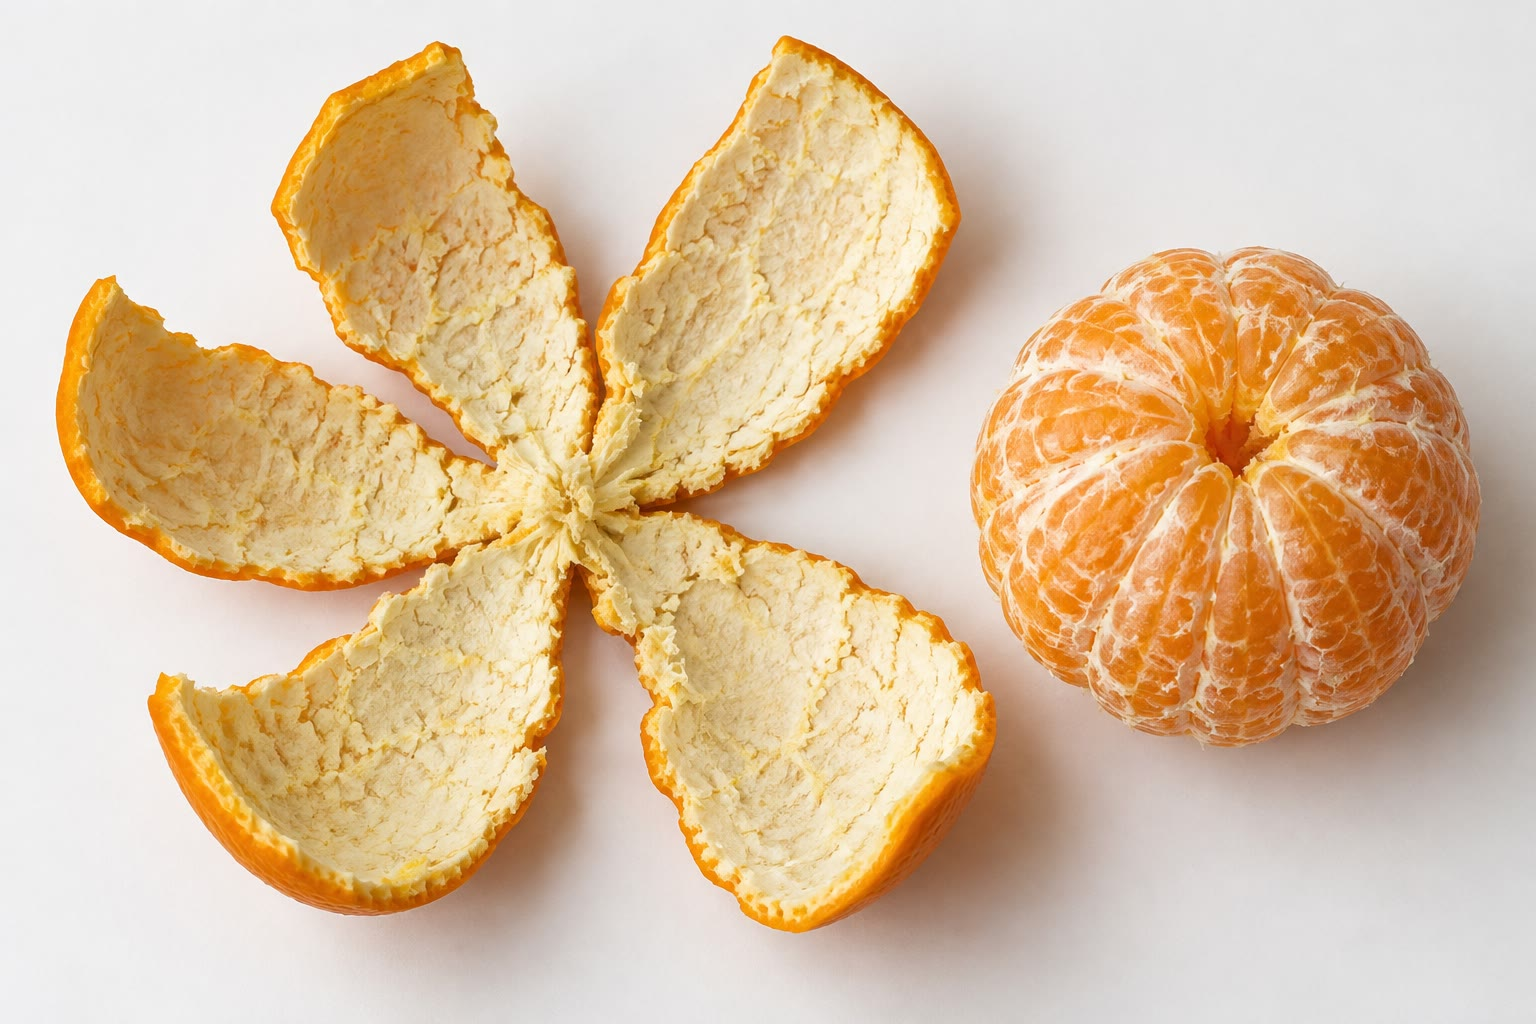
\includegraphics[width=0.4\linewidth]{images/book1/ai/g3-orange-peel.jpg}

{\small De schil van een sinaasappel ligt nooit plat zonder te scheuren.}
\end{omfigure}

\begin{remark}[De kaart en de globe zijn het oneens]\label{rem:g3:continents-and-oceans:disagree}
Op deze \omterm{def:g3:continents-and-oceans:world-map}{wereldkaart} lijkt Antarctica een van de grootste \omterm{def:g3:continents-and-oceans:continent}{continenten},
uitgerekt langs de hele onderrand. Op de \omterm{def:g3:continents-and-oceans:globe}{globe} is het een ronde landmassa,
kleiner dan Zuid-Amerika. Dicht bij de \omterm{def:g3:continents-and-oceans:poles}{polen} rekt een platte \omterm{def:g2:drawing-to-map:map}{kaart} het land
flink uit. Dicht bij de \omterm{def:g3:continents-and-oceans:equator}{evenaar} rekt hij het maar heel weinig. Wil je de
grootte van twee plekken ver van de \omterm{def:g3:continents-and-oceans:equator}{evenaar} vergelijken, dan vertelt de
\omterm{def:g3:continents-and-oceans:globe}{globe} de waarheid.
\end{remark}

\begin{method}[Een wereldkaart lezen]\label{met:g3:continents-and-oceans:reading}
Op een \omterm{def:g3:continents-and-oceans:world-map}{wereldkaart} zoals deze:
\begin{enumerate}
  \item ligt het noorden boven en het zuiden onder; de \omterm{def:g3:continents-and-oceans:poles}{Noordpool} is de hele
        bovenrand en de \omterm{def:g3:continents-and-oceans:poles}{Zuidpool} de hele onderrand;
  \item is de \omterm{def:g3:continents-and-oceans:equator}{evenaar} de lijn dwars door het midden: alles erboven ligt op
        het \omterm{def:g3:continents-and-oceans:equator}{noordelijk halfrond}, alles eronder op het \omterm{def:g3:continents-and-oceans:equator}{zuidelijk halfrond};
  \item zijn de linker- en de rechterrand dezelfde lijn op de \omterm{def:g3:continents-and-oceans:globe}{globe}: een
        schip dat aan de rechterrand van de \omterm{def:g2:drawing-to-map:map}{kaart} vaart, komt links weer
        terug.
\end{enumerate}
\end{method}

\section{Oefeningen}

\begin{exercise}[$\star$]\label{exo:g3:continents-and-oceans:1}
Noem de zeven \omterm{def:g3:continents-and-oceans:continent}{continenten}. Welk is het grootste? Welk is het kleinste?
\end{exercise}

\begin{exercise}[$\star$]\label{exo:g3:continents-and-oceans:2}
Noem de vijf \omterm{def:g2:water-on-earth:ocean}{oceanen}. Welke is de grootste? Welke is de kleinste?
\end{exercise}

\begin{exercise}[$\star$]\label{exo:g3:continents-and-oceans:3}
Schrijf over en vul in met ``\omterm{def:g3:continents-and-oceans:poles}{Noordpool}'', ``\omterm{def:g3:continents-and-oceans:poles}{Zuidpool}'' of ``\omterm{def:g3:continents-and-oceans:equator}{evenaar}'': de
\dots{} ligt bovenaan op een \omterm{def:g3:continents-and-oceans:globe}{globe}; de \dots{} ligt onderaan; de \dots{}
loopt helemaal om het midden heen.
\end{exercise}

\begin{exercise}[$\star$]\label{exo:g3:continents-and-oceans:4}
Noordelijk of \omterm{def:g3:continents-and-oceans:equator}{zuidelijk halfrond}? Europa; Australië; Antarctica;
Noord-Amerika.
\end{exercise}

\begin{exercise}[$\star$]\label{exo:g3:continents-and-oceans:5}
Welke \omterm{def:g2:water-on-earth:ocean}{oceaan} ligt rond de \omterm{def:g3:continents-and-oceans:poles}{Noordpool}? Welke \omterm{def:g2:water-on-earth:ocean}{oceaan} ligt rond
Antarctica?
\end{exercise}

\begin{exercise}[$\star\star$]\label{exo:g3:continents-and-oceans:6}
Welke \omterm{def:g2:water-on-earth:ocean}{oceaan} steek je over om van Afrika naar Zuid-Amerika te gaan? Van
Australië naar Zuid-Amerika, naar het oosten? Van Afrika naar Australië?
\end{exercise}

\begin{exercise}[$\star\star$]\label{exo:g3:continents-and-oceans:7}
Sam woont in een land waar het het hele jaar door warm is. Bo woont op een
onderzoeksstation waar het het hele jaar door vriest. Een van hen woont bij
de \omterm{def:g3:continents-and-oceans:equator}{evenaar}, de ander bij een \omterm{def:g3:continents-and-oceans:poles}{pool}. Wie woont waar?
\end{exercise}

\begin{exercise}[$\star\star$]\label{exo:g3:continents-and-oceans:8}
Lena laat de \omterm{def:g3:continents-and-oceans:globe}{globe} 10 keer draaien. Haar vinger komt 7 keer op de \omterm{def:g2:water-on-earth:ocean}{zee}
terecht. Hoe vaak komt hij op het land? Had je dat verwacht? Waarom?
\end{exercise}

\begin{exercise}[$\star\star$]\label{exo:g3:continents-and-oceans:9}
Op de \omterm{def:g3:continents-and-oceans:world-map}{wereldkaart} op pagina~\pageref{fig:g3:continents-and-oceans:world-map}
staat de Stille \omterm{def:g2:water-on-earth:ocean}{Oceaan} twee keer. Waarom? Heeft de echte Aarde twee Stille
\omterm{def:g2:water-on-earth:ocean}{Oceanen}?
\end{exercise}

\begin{exercise}[$\star\star\star$]\label{exo:g3:continents-and-oceans:10}
Tom zegt: ``Op de \omterm{def:g3:continents-and-oceans:world-map}{wereldkaart} is Antarctica langer dan Azië, dus is
Antarctica het grootste \omterm{def:g3:continents-and-oceans:continent}{continent}.'' Heeft Tom gelijk? Gebruik de lijst
van de \omterm{def:g3:continents-and-oceans:continent}{continenten} van groot naar klein, en zeg waarom de \omterm{def:g3:continents-and-oceans:world-map}{wereldkaart} hem
voor de gek houdt.
\end{exercise}
